\chapter{Event Spotting on Video}
\label{chap:event}

\section{Introduction}
As mentioned in chapter \ref{chap:intro}, our ultimate aim was to find all the events in the search video $(\mathcal{V})$ which are similar to the event in given query $(\mathcal{Q})$  for a given video ($\mathcal{V}$) and a query $(\mathcal{Q})$. Since video is temporal sequence we have to model temporal dependencies
in the data at sub-event level. 

Dynamic time warping is well known for it's ability to compare two time dependent sequences. Intuitively, the sequences are warped in a nonlinear fashion to match each other. Even though DTW was developed for compare different speech patterns in ASR (Automatic Speech Recognition), nowadays DTW has been applied to other fields \cite{muller2007information}.  So we decided to make use of DTW for comparing (and hence spotting events) in Query and Search Video.

Now we have to extract effective features from video sequence so that features will be able to describe events  in video. We decided to make use of Deep Neural Network for extracting these features. 

In this chapter, We will fist discuss why we preferred  DNN over classical feature extractors. In Section \ref{sec:event:unsupervised}, we go through different unsupervised methods attempted to answer the question \textit{``Will any unsupervised Deep Learning Techniques work for feature extraction ?"}. Later in section \ref{sec:event:supervised}, we go through experiments which uses supervised CNNs  

\section{Why Deep Neural Networks?}
\label{sec:event:why}
We have to capture underlying temporal structures of actions (i.e. intra-dependencies) through feature representations. Some of classical features in videos are SIFT(Scale-invariant feature transform), HOG (Histogram of oriented gradients), Optical Flow, HOF (Histograms of flow orientations), HOG3D (Histograms of 3D gradients), MBH (motion boundary histograms). These classical feature extraction requires high amount of computaion \cite{baker2011database,chatfield2011devil}. This time-consuming process of feature extraction limits the speed of testing and hence limiting the scope of real time applications.

In recent years, deep learning has produced remarkable results and significantly outperformed state-of-the-art the classical methods \cite{KarpathyCVPR14}. Deep Neural Networks (DNNs) is able to learning the feature representation directly from input and hence bring significant performance boosting (refer chapter \ref{chap:dnn}). Moreover, bottleneck features generated from deep neural networks (Deep Bottleneck Features) are found as better features in automatic speech recognition (ASR) systems \cite{yu2011improved,gehring2013extracting}.

\section{Unsupervised Methods}
\label{sec:event:unsupervised}
Our initial approach was to find out \textit{``Will any unsupervised Deep Learning Techniques work for feature extraction ?"}. Experiments are done on the OSUPEL basketball dataset \cite{brendel2011probabilistic}.The OSUPEL basketball dataset contains videos of drills and small basketball games. Since these videos were shot in a real-world setting it contains challenges like slow and sudden camera motion, motion blur of fast actions, inter-player occlusions, and varying illumination. Resolution of data set is $960 \times 540$ pixels and frame rate is $29$fps.

In this section we go through different unsupervised Deep Neural Network methods that has been experimented. 

\subsection{Deep Belief Network} 
We took complete video and reduced resolution to $256 \times 144$ pixels (from $960 \times 540$). Then each frame is fed to a \textit{Deep Belief Network (DBN)} which tries to reduce it's dimensionality. Different DBNs with different sizes of deep bottleneck features (400,1000 and 2000) were analysed. But we encountered a problem: the features we obtained were somewhat random. We found that the large size of the weight matrix is the reason behind this issue. To train such a big network, we need a big data-set.

\subsection{DBN on DCT Coefficients}
Since our previous attempt failed as the input dimension was too big, we decided to make use of Discrete Cosine Transform (DCT).Advantage of DCT can be implemented using a fast algorithm and is commonly used for dimensionality reduction in images/videos \cite{er2005high}. Reduced resolution video ($256 \times 144$) is taken and DCT is computed for each frame. The low-frequency coefficients of DCT is taken (top 1500) and is normalised with respect to mean. Then we used Deep Belief Network which tries to reduce dimensionality (to 400/200).

But it was found that DBN features yields same outputs, irrespective of the input, if we use more than one layer. With a single layer Restricted Boltzmann machine (first Layer is Gaussian-Bernoulli layer), we are getting some variation but not enough for identifying the events.\\


\begin{figure}
        \centering
        \begin{subfigure}[b]{\textwidth}
        			\centering
                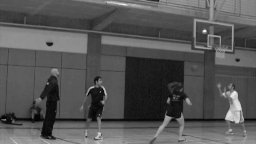
\includegraphics[scale=1]{./imgs/Original.png}
                \caption{Original frame}
                \label{fig:original}
        \end{subfigure}%
        %newline
        
        \begin{subfigure}[b]{0.45\textwidth}
        		\centering
        		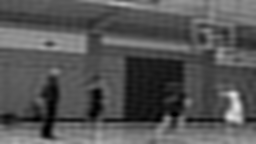
\includegraphics[scale=1]{./imgs/DCT.png}
        		\caption{Reconstructed frame from top 1500 DCT coefficients}
        		\label{fig:dct}
        \end{subfigure}
        ~%~ %add desired spacing between images, e. g. ~, \quad, \qquad, \hfill etc.
        \begin{subfigure}[b]{0.45\textwidth}
        			\centering
                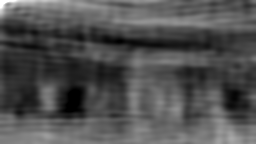
\includegraphics[scale=1]{./imgs/DBN.png}
                \caption{Reconstructed frame from DBN features (single layer)}
                \label{fig:dbn}
        \end{subfigure}
        \caption{ A XXXXXXXXX of DBN features}
        \label{fig:dct+dbn}
\end{figure}\\

\subsection{SdA on DCT Coefficients}
Instead of using DBN to reduce the dimensionality, we tried to use \textit{Stacked Denoising Auto-encoder (SdA)} for same. It also failed to capture features which are abstract representation of events in the video.\\
Since SdA tries to learn weights so that reconstruction error is less and most of DCT low frequency Coefficients across frames having less variance, SdA tries to learn common features instead of varying features.

\subsection{Using DCT and GMM}

We build smaller GMMs (4 - 50 mixtures), and trained them with some of the videos. We then took the responsibility of each frame in the search and query video. As the query contains only one event, we represented each query as a single vector (mean of the responsibilities of all frames in the query). Inner product of each search video vector (corresponding to each frame of the search video) with representative vector of query video is taken. Finally, all the continuous frames of length at-least half of that of the query with all inner products greater than a threshold, are considered similar events. With 5 mixtures and 0.65 as the threshold, we captured most events but also captured a lot of false positives.\\


\section{Supervised Methods}
\label{sec:event:supervised}
\subsection{3dCNN with color map feature}
\subsection{CNN with color map feature}
\subsection{CNN with frame-difference and edge detection}

\section{Summary}
